% !TeX encoding=utf-8
\documentclass[a4paper]{feidippp}
\usepackage[pdftex]{graphicx}
\DeclareGraphicsExtensions{.pdf,.png.,mps.,jpg}
\graphicspath{{figures/}}

\usepackage[utf8]{inputenc}
\usepackage[T1]{fontenc}
\usepackage[slovak]{babel}

\usepackage{lmodern}

\usepackage{amsmath,amssymb,amsfonts}

\def\figurename{Obrázok}
\def\tabname{Tabuľka}



%\usepackage[dvips]{graphicx}
%\DeclareGraphicsExtensions{.eps}



%\usepackage[pdftex]{hyperref}   %% tlac !!!
\usepackage[pdftex,colorlinks,citecolor=magenta,bookmarksnumbered,unicode,pdftoolbar=true,pdfmenubar=true,pdfwindowui=true,bookmarksopen=true]{hyperref}
\hypersetup{%
baseurl={http://www.tuke.sk/sevcovic},
pdfcreator={pdfcsLaTeX},
pdfkeywords={Používateľská priručka },
pdftitle={Šablóna na písanie DP na FEI TU v~Košiciach},
pdfauthor={Ján Buša, Ladislav Ševčovič},
pdfsubject={Ako napísať peknú DP}
}

% Citovanie podla mena autora a roku
%\usepackage[numbers]{natbib}
\usepackage{natbib} \citestyle{chicago}

%\usepackage{mathptm} %\usepackage{times}

\katedra{Laboratórium priemyselného inžinierstva}
\department{Laboratory of Industrial Engineering}
\odbor{Experimentálna fyzika}
\autor{Ján Zelený}
\veduci{Doc.~Ing.~Vojtech Čierny, CSc.}
\konzultant{Ing. Matej Biely, PhD.}
\nazov{Optimalizácia písania diplomových prác na našej fakulte}
\kratkynazov{Optimalizácia písania DP}
\nazovprogramu{ODYSSEUS}
\klucoveslova{optimalizácia, diplomová práca, písanie}
\title{The optimization of the diploma writing at our faculty}
\keywords{optimization, diploma, writing}
\datum{30. 4. 2016}



\begin{document}
\bibliographystyle{dcu}



\titulnastrana

\newpage


\tableofcontents



\newpage

\setcounter{page}{1}

\section{Funkcia programu}

Popis, čo daný program vykonáva, oblasti použitia, charakteristika riešených úloh prostredníctvom programu, mená autorov, údaje o~dodávatelovi, licencné podmienky a~pod., prehlad o~dokumentácii k~programu. 


\section{Súpis obsahu dodávky}

Predpokladom je, že je k~dispozícii zhotovený program v~binárnej forme s~inštalacnými podporami. Potrebné  uviesť:
\begin{itemize}
\item počet médií so zoznamom súborov, ktoré obsahuje inštalacné médium;
\item zoznam dokumentácie (Používateľská príručka, atď.).
\end{itemize}

\section{Inštalácia programu}

\subsection{Požiadavky na technické prostriedky}

Typ počítača, požadovaná veľkosť operačnej pamäte, potrebný diskový priestor, prídavné zariadenia, atď.

\subsection{Požiadavky na programové prostriedky}
Operačný systém, obslužné programy, knižnice, atď.

\subsection{Vlastná inštalácia}

Postup inštalácie programu.

\subsection{Popis štruktúry programu}

Uviesť údaje o~moduloch  programu a~ich spolupráci pri aktivácii programu a~taktiež             o~spoluprácu s~inými programami. Po jednotlivých krokoch rozpísať postup aj s~očakávanými  dobrými a~chybovými odozvami.

V~texte môžu byt použité obrázky a~tabuľky  podľa nasledujúcich príkladov:

\begin{figure}[!ht]
\centering 
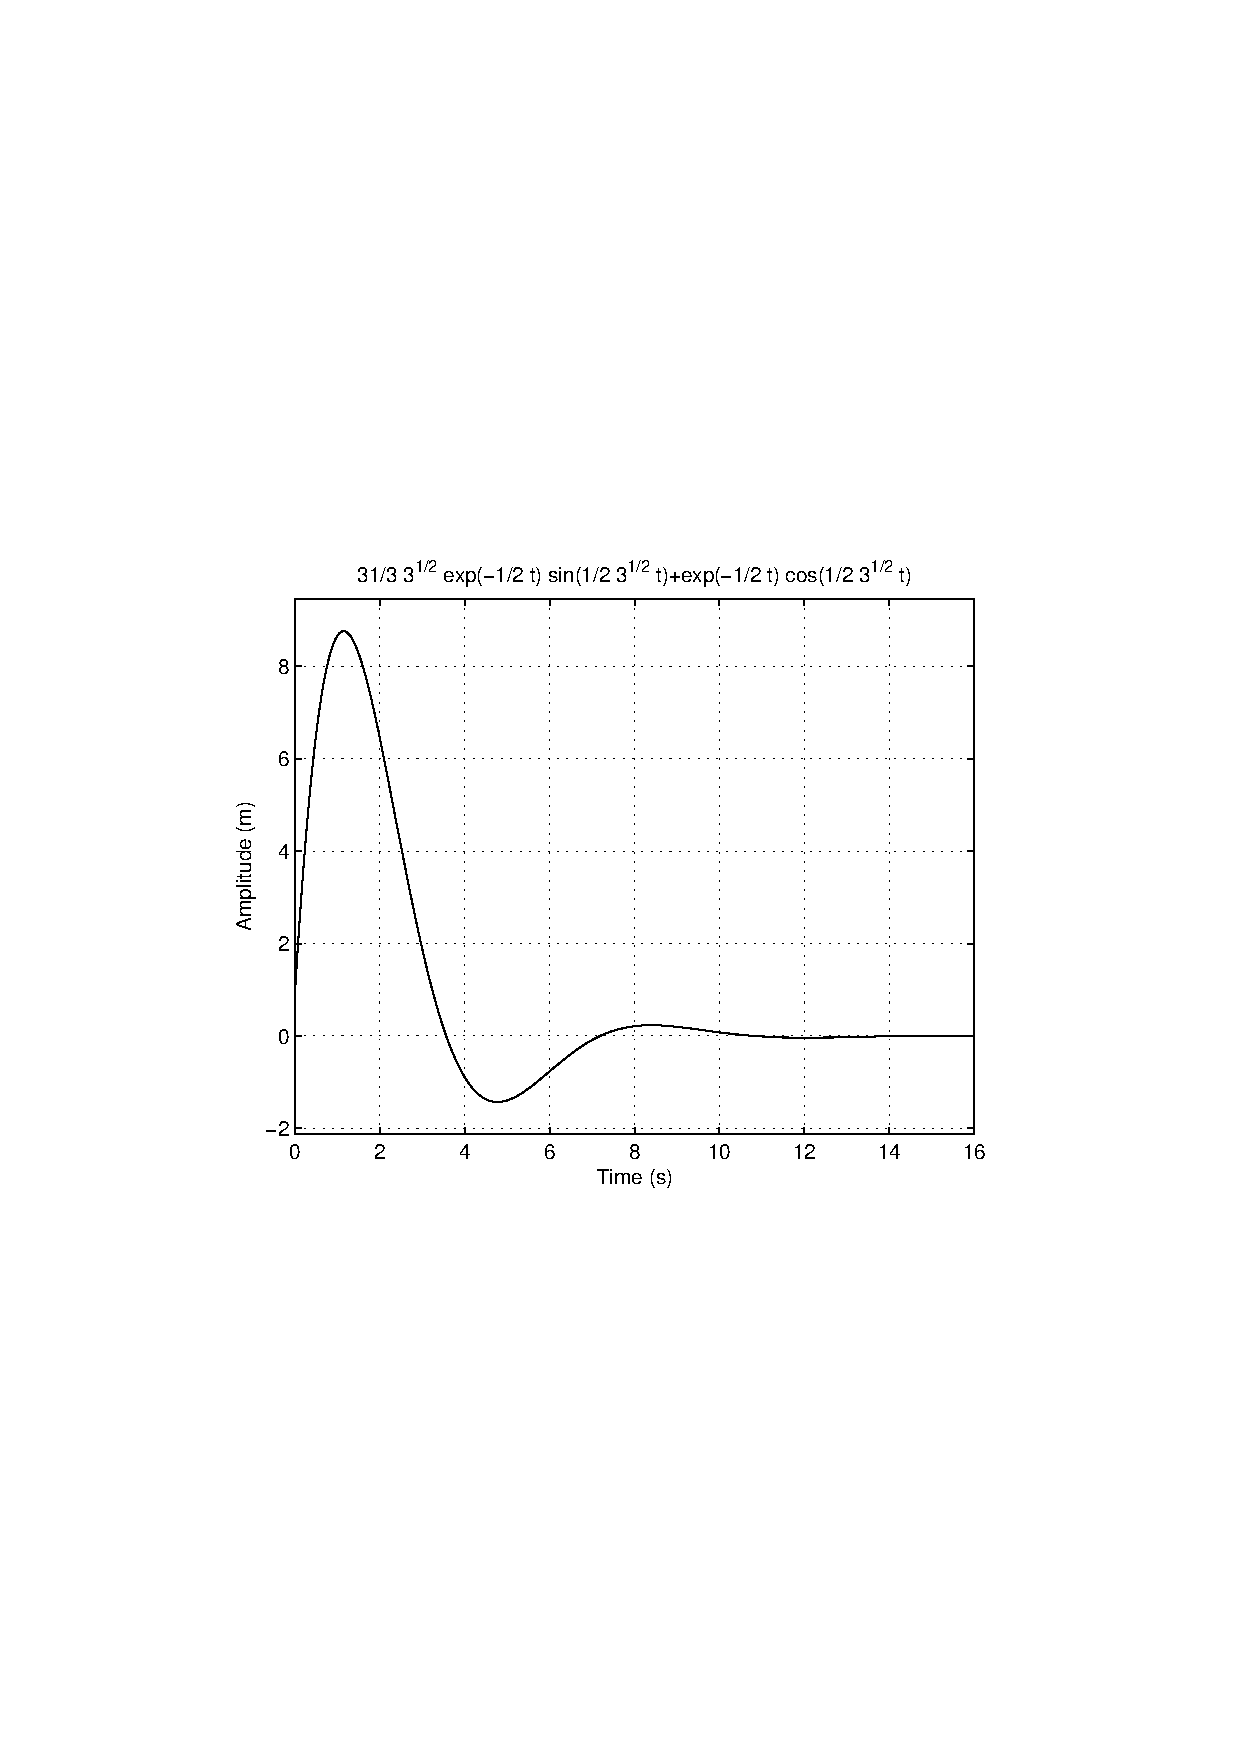
\includegraphics[width=0.5\textwidth]{tlmosc}
\caption{Tlmené oscilácie}\label{o:1}
\end{figure}

Obrázok by mal byt podľa možnosti centrovaný. Pri jeho popisovaní v~texte treba použiť odkazy na obrázok v~tvare obrázok \ref{o:1}.

\begin{table}[!ht]\caption{Prehľad jednotiek}\label{t:1}
\smallskip
\centering
\begin{tabular}{|l|c|} \hline
Názov	& [\,jednotka] \\ \hline
Napätie & $\mu$V \\ \hline
\end{tabular}	
\end{table}


Tabuľka by mala byť podľa možnosti centrovaná. Pri jej popisovaní v~texte treba použiť odkazy na tabuľku v~tvare tabuľka \ref{t:1}.
Na číslovanie obrázkov, resp. tabuliek treba použiť desatinné triedenie, prvé číslo odpovedá číslu kapitoly, resp. podkapitoly.


\subsection{Popis správ pre systémového programátora}

Uviest texty správ, ktoré sa vypisujú pocas cinnosti programu, príciny týchto správ, popis programu cinnosti, ktoré je potrebné po týchto správach vykonat.

\section{Použitie programu}
Stručný popis použitia programu.

\subsection{Popis dialógu s~používateľom}

Napr. pomocou stromu dialógu.

\subsection{Popis funkcií a~podfunkcií programu}

Popis jednotlivých funkcií a~podfunkcií programu z~používateľského pohľadu (služby programu) s~využitím napr. \uv{hardcopy} obrazovky.

\section{Popis vstupných, výstupných a~pracovných súborov}

Napr. formáty súborov, atd.

\section{Obmedzenia programu}

Zoznam obmedzení programu.

\section{Chybové hlásenia}

Chybové hlásenia vlastné pre daný aplikacný program.

Chybové hlásenia súvisiace s~OS, Štandard. p.~p., \dots).

\section{Príklad použitia}

Príklad použitia programu.

\section{Popis demo-verzie}

Popis demo-verzie. V~prípade, že navrhovaný program je demo-verzia.

\addcontentsline{toc}{section}{\numberline{}Zoznam obrázkov}
\listoffigures

\addcontentsline{toc}{section}{\numberline{}Zoznam tabuliek}
\listoftables


\def\refname{Zoznam použitej literatúry}
\addcontentsline{toc}{section}{\numberline{}Zoznam použitej literatúry}

\begin{thebibliography}{999}
\harvarditem{Barančok et al.}{1995}{barancok}
BARANČOK, D. et al. 1995. \emph{The effect of semiconductor surface treatment on LB film/Si interface.} In:~Physica Status Solidi /a/,  ISSN 0031-8965, 1995, vol. 108, no.2, pp. K~87\,--\,90

\harvarditem{Gonda}{2001}{gonda}
GONDA, V. 2001. \emph{Ako napísať a~úspešne obhájiť diplomovú prácu.} Bratislava : Elita, 2001, 3.~doplnené a~prepracované vydanie, 120~s. ISBN 80-8044-075-1

\harvarditem{Jadr. fyz. a~tech.}{1985}{slovnik}
\emph{Jadrová fyzika a~technika: Terminologický výkladový slovník.} 2.~rev.~vyd. Bratislava : ALFA, 1985. 235 s. ISBN 80-8256-030-5

\harvarditem{Katuščák}{1998}{kat}
KATUŠČÁK, D. \emph{Ako písať vysokoškolské a~kvalifikačné práce.} Bratislava : Stimul, 1998, 2.~doplnené vydanie. 121~s. ISBN 80-85697-82-3

%\harvarditem{Sýkora a~i.}{1980}{sykora}
%SÝKORA, F. a~iní. 1980. \emph{Telesná výchova a~šport.} 1.~vyd. Bratislava : SPN, 1980. 35 s. ISBN 80-8046-020-5

\harvarditem{Lamoš a~Potocký}{1989}{lamos}
LAMOŠ, F. -- POTOCKÝ, R. 1989. \emph{Pravdepodobnosť a~matematická štatistika.} 1.~vyd. Bratislava : Alfa, 1989. 344 s. ISBN 80-8046-020-5

%\harvarditem{Sýkora a~i.}{1980}{sykora}
%SÝKORA, F. a~iní. 1980. \emph{Telesná výchova a~šport.} 1.~vyd. Bratislava : SPN, 1980. 35 s. ISBN 80-8046-020-5

\harvarditem{Lamoš a~Potocký}{1989}{lamos}
LAMOŠ, F. -- POTOCKÝ, R. 1989. \emph{Pravdepodobnosť a~matematická štatistika.} 1.~vyd. Bratislava : Alfa, 1989. 344 s. ISBN 80-8046-020-5


\end{thebibliography}


\end{document}


